\section{Quadrature error of the trapezoidal rule}\label{app::trapezoidal}
We employ the method of contour integrals~\cite{Donaldson1972SINUA,trefethen2014Rev} to derive a precise estimation for the error in  {the} trapezoidal rule when discretizing Eqs.~\eqref{eq:ewald2d-intform1} and \eqref{eq::J02}. Consider the integral
\begin{equation}\label{eq::A.1}
I=\int_{-\infty}^{\infty }\frac{e^{-(a^2+t^2)}}{a^2+t^2}e^{\i b t}dt,
\end{equation}
where $a\geq 0$ and $b\in\mathbb{R}$. We approximate $I$ using a $(2M+1)$-point trapezoidal rule:
\begin{equation}
I_{M,\xi}=\xi\sum_{j=-M}^{M}\frac{e^{-a^2-(j\xi)^2}}{a^2+(j\xi)^2}e^{\i b j\xi},
\end{equation}
where $\xi>0$ is the step size, and we define the remainder as $E_{M,\xi}:=I-I_{M,\xi}$. Note that the integrand of $I$ has two simple poles at $t_{\pm}=\pm \i a$. Let $\Gamma_{\pm}$ be two positively/negatively oriented rectangular contours with vertices $(M+1/2)\xi\pm\i a^*$, $-(M+1/2)\xi\pm\i a^*$, $(M+1/2)\xi$, and $-(M+1/2)\xi$ (see Fig.~\ref{fig:Trapezoidal}). We enforce $a^*>a$ so that $\Gamma_{\pm}$ encloses both the interval $[-M \xi,M \xi]$ and the pole $t_{\pm}$. By following the approach given in~\cite{Donaldson1972SINUA} and applying Cauchy's theorem, we can derive an estimate for $E_{M,\xi}$ in the limit $M\rightarrow \infty$:
\begin{equation}
E_{M,\xi}=\int_{\Gamma_++\Gamma_-}\frac{e^{-(a^2+t^2)+\i b t}}{a^2+t^2}\varphi(t)dt-2\pi\i \text{Res}\left[\frac{e^{-(a^2+t^2)+\i b t}}{a^2+t^2}\varphi(t),\pm \i a\right],
\end{equation}
where
\begin{align}
\varphi(t)=\begin{cases}
\dfrac{1}{1-e^{2\pi\i t/\xi}},\,\quad &\text{Im}(t)<0,\\[1em]
-\dfrac{1}{1-e^{-2\pi\i t/\xi}},\,\quad&\text{Im}(t)>0,
\end{cases}
\end{align}
is related to the characteristic function of the trapezoidal rule, and $\text{Res}[f(t),t_0]$ denotes the residue of a function $f$ at a pole $t_0$. Since the contributions from the vertical sides of $\Gamma_{\pm}$ vanish in the limit $M\rightarrow \infty$ and by using residue calculus, we have
\begin{equation}\label{eq::A.5}
E_{M,\xi}=\left(\int_{-\infty+\i a^*}^{\infty+\i a^*}-\int_{-\infty-\i a^*}^{\infty-\i a^*}\right)\frac{e^{-(a^2+t^2)+\i b t}}{a^2+t^2}\varphi(t)dt+\frac{\pi}{a}\frac{e^{-ab}+e^{ab}}{1-e^{2\pi a/\xi}}.
\end{equation}
In Eq.~\eqref{eq::A.5}, the last term can be considered as the residue correction of the rule, while the remainder integral along $\text{Im}(t)=a^*$ can be estimated as
\begin{equation}
\begin{split}
\left|\int_{-\infty+\i a^*}^{\infty+\i a^*}\frac{e^{-(a^2+t^2)+\i b t}}{a^2+t^2}\varphi(t)dt\right|&\leq e^{(a^*)^2-a^2-a^*b-2\pi a^*/\xi}\int_{-\infty}^{\infty}\frac{|a^2+(t+\i a^*)^2|^{-1}e^{-t^2}}{\left|1-e^{2\pi\i t/\xi-2\pi a^*/\xi}\right|}dt\\
&\leq\frac{\sqrt{\pi}e^{(a^*)^2-a^2-a^*b-2\pi a^*/\xi}}{(a^*)^2-a^2}.
\end{split}
\end{equation}

To obtain a closed formula, it is necessary to determine the extremum of the exponent under the condition $a^*>a>0$. Since the range of $a$ is not specified, we can safely choose $a^*=\pi/\xi+b/2$ if $\pi/\xi+b/2>a$, and $a^*=\sqrt{a^2+1}$ otherwise. This choice ensures a decay rate of at least $\sim\mathcal{O}(e^{-\text{sign}(\pi/\xi+b/2)|\pi/\xi+b/2|^2})$, where $\text{sign}(t)=1$ if $t> 0$, $\text{sign}(t)=0$ if $t=0$, and $\text{sign}(t)=-1$ otherwise. By following a similar procedure, we can derive that the integral along $\text{Im}(t)=-a^*$ in Eq.~\eqref{eq::A.5} decays with order $\mathcal{O}(e^{-\text{sign}(\pi/\xi-b/2)|\pi/\xi-b/2|^2})$. Consequently, we can conclude that
\begin{equation}
E_{M,\xi}=\frac{\pi}{a}\frac{e^{-ab}+e^{ab}}{1-e^{2\pi a/\xi}}+E_{\text{err}},
\end{equation}
where the remainder error term can be estimated as 
\begin{equation}\label{eq::A.8}
|E_{\text{err}}|\sim \mathcal{O}(e^{-\text{sign}(\pi/\xi-|b|/2)\left|\pi/\xi-|b|/2\right|^2}).
\end{equation}

\begin{figure}[!ht]
    \begin{center}
    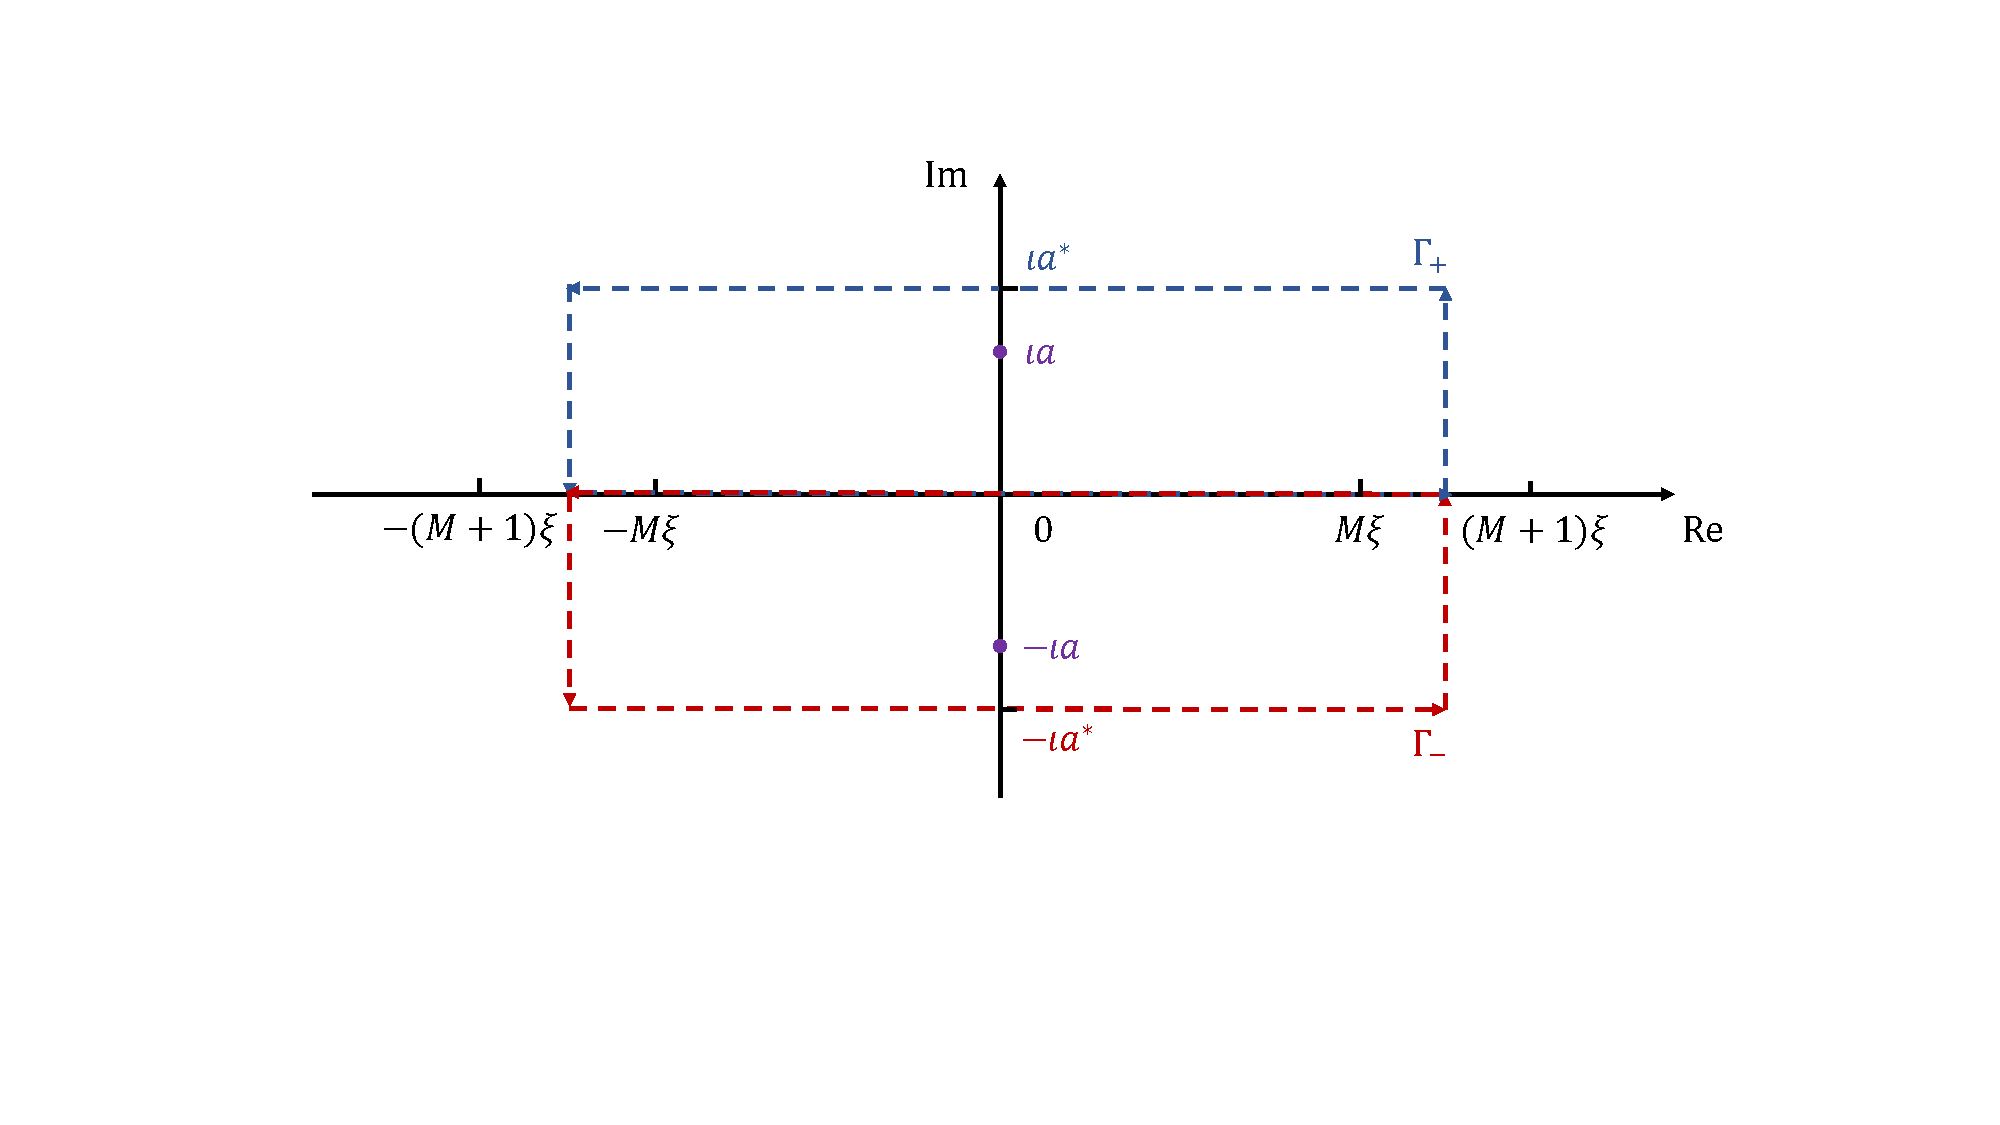
\includegraphics[width=0.8\textwidth]{figs/Trapezoidal.pdf}
    \caption{Integration contours in the error estimation of trapezoidal rule.}
    \label{fig:Trapezoidal}
    \end{center} 
\end{figure}